\chapter{Getting Started}
\label{chap:starting}

\section{Hello Proofs}

The first and basic step in using Why3 is to write a suitable input
file. When one wants to learn a programming language, you start by
writing a basic program. Here we start by writing a file containing a
basic set of goals. 

Here is our first Why3 file, which is the file
\texttt{examples/hello\_proof.why} of the distribution.
\verbatiminput{../examples/hello_proof.why} Any declaration must occur
inside a theory, which is in that example called TheoryProof and
labelled with a comment inside double quotes. It contains three goals
named $G_1,G_2,G_3$. The first two are basic propositional goals,
whereas the third involves some integer arithmetic, and thus it
requires to import the theory of integer arithmetic from the Why3
standard library, which is done by the \texttt{use} declaration above.

We don't give more details here about the syntax and refer to
Chapter~\ref{chap:syntax} for detailed explanations. In the following,
we show how this file is handled in the Why3 GUI
(Section~\ref{sec:gui}) then in batch mode using the \texttt{why3}
executable (Section~\ref{sec:batch}) .


\section{Getting Started with the GUI}
\label{sec:gui}

The graphical interface allows to browse into a file or a set of
files, and check the validity of goals with external provers, in a
friendly way. This section presents the basic use of this GUI. Please
refer to Section~\ref{sec:ideref} for a more complete description.

\begin{figure}[tbp]
  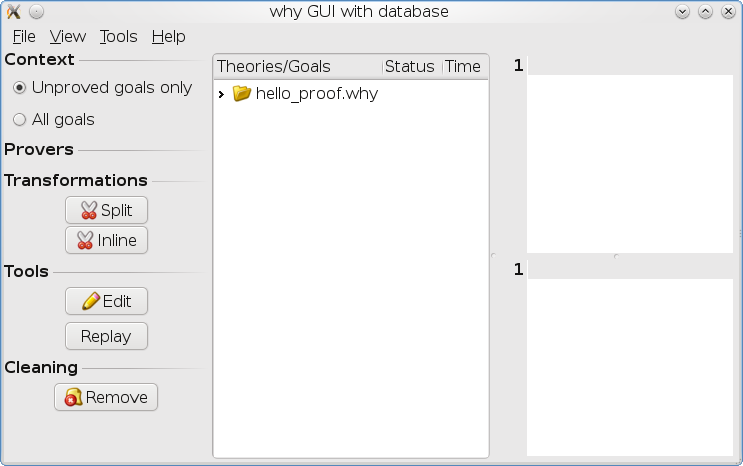
\includegraphics[width=\textwidth]{gui1.png}
  \caption{The GUI when started the very first time}
  \label{fig:gui1}
\end{figure}

The GUI is launched on the file above as follows.
\begin{verbatim}
why3ide hello_proof.why
\end{verbatim}
When the GUI is started for the first time, you should get a window
which look like the screenshot of Figure~\ref{fig:gui1}. First of all,
the left row is a tool bar which provide different actions to apply on
goals. In this case, the section ``Provers'' is empty, which means
that you did not perform prover detection yet. You should do it now
using the menu \textsf{File/Detect provers}. Second, the middle part
is a tree view that allows to browse inside the theories. Initially,
the item of this tree are closed. You should now expand this view
using the menu \textsf{View/Expand all} or its shortcut
\textsf{Ctrl-E}. This should result is something like the screenshot of Figure~\ref{fig:gui2}.

\begin{figure}[tbp]
  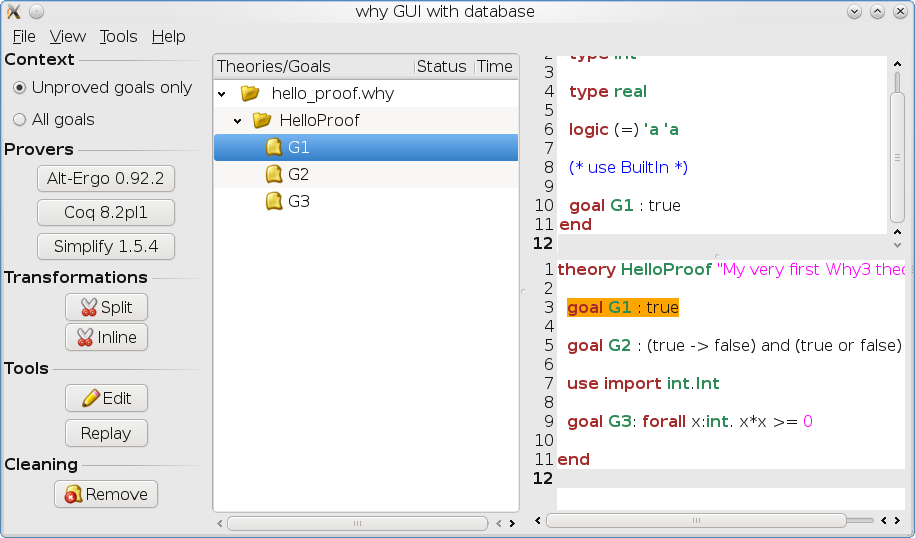
\includegraphics[width=\textwidth]{gui2.png}
  \caption{The GUI with provers detected and tree view expanded}
  \label{fig:gui2}
\end{figure}

In the tree view, we have now a strctured view of the file: this file
contains one theory, itself containg three goals. In
Figure~\ref{fig:gui2}, we also clicked on the row corresponding to
goal $G_1$. The \emph{task} associated with this goal is then
displayed on the top right, and the corresponding part of the input
file is shown on the bottom right part.

Notice also that three provers where detected, and are now shown as
button in the ``provers'' section of the left toolbar. In that case,
detected provers are Alt-Ergo~\cite{ergo}, Coq~\cite{CoqArt} and
Simplify~\cite{simplify05}. 

You are now ready to call these provers on the goals. Whenever you
click on a prover button, this prover is called on the goal selected
in the tree view. You can even select several goals at a time, either
by using multi-selection (typically by clicking while pressing the
\textsf{Shift} or \textsf{Ctrl} key) or by selecting the parent theory
or the parent file. Let us now select the theory ``HelloProof'' and
click on the \textsf{Simplify} button. After a short time, you should
get the display of Figure~\ref{fig:gui3}.

\begin{figure}[tbp]
  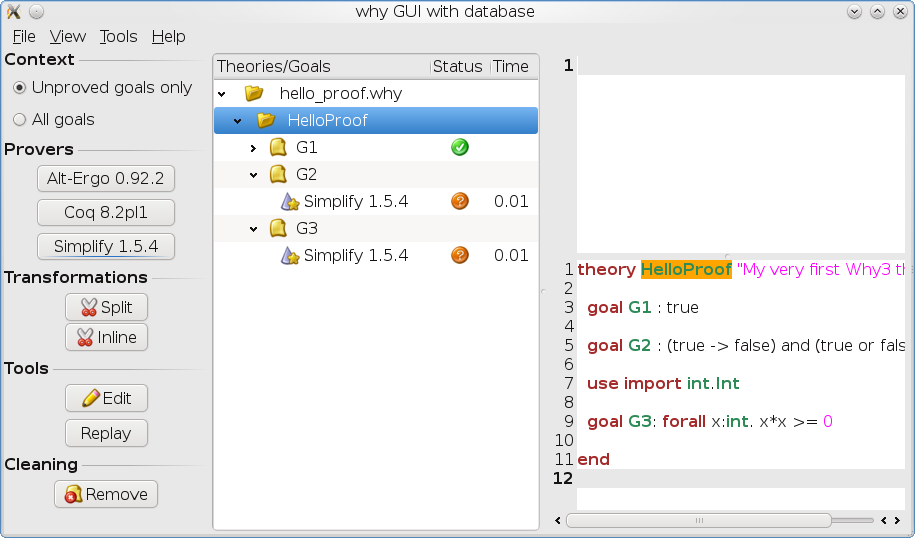
\includegraphics[width=\textwidth]{gui3.png}
  \caption{The GUI after Simplify prover is run on each goal}
  \label{fig:gui3}
\end{figure}


\section{Getting Started with the Why3 Command}
\label{sec:batch}

The why3 command allows to check the validity of goals with external
provers, in batch mode. This section presents the basic use of this
tool. Refer to Section~\ref{sec:why3ref} for a more complete
description.





%%% Local Variables:
%%% mode: latex
%%% TeX-PDF-mode: t
%%% TeX-master: "manual"
%%% End:
